\documentclass[a4paper,12pt,twoside]{proyectotanquesecci}
\usepackage{graphicx}
\usepackage{eqparbox}
\usepackage[tight,footnotesize]{subfigure}
\usepackage{hyperref}
\usepackage[spanish]{babel}
\usepackage[utf8]{inputenc}
\hyphenation{op-tical net-works semi-conduc-tor}
\usepackage{algpseudocode}
\usepackage{algorithm}
\usepackage{colortbl}
\usepackage{fancyhdr}
\usepackage{anysize}
\marginsize{3cm}{3cm}{2.5cm}{2.5cm}
\title
{
\textbf{Capítulo de libro del grupo de control (M-ECCI)}\\
\vspace{3cm}
{\large 
Sergio Andres Acosta Herrera \\
Dayanis Andrea Suarez Rodriguez\\
Omar Andres Castañeda Goméz\\
Sergio Agustin Oñate Sierra\\}
\vspace{1cm}
\textbf{Director}\\
{\large Ing. Jhon Fredy Bayona Navarro M.Sc.}\\
\vspace{2cm}
{\large Bogotá D.C.}
}
\pagestyle{fancy}
\renewcommand{\chaptermark}[1]{\markboth{#1}{}}
\renewcommand{\sectionmark}[1]{\markright{#1}}
\fancyhf{}
\lhead[\small{\thepage}]%
      {\small{\rightmark}}
\rhead[\small{\leftmark}]%
      {\small{\thepage}}
\cfoot{}
\lfoot[\small{M-ECCI}]%
      {\small{Trabajo de Grado}}
\rfoot[\small{Trabajo de Grado}]%
      {\small{M-ECCI}}
\begin{document}
\maketitle
\renewcommand{\contentsname}{Tabla de Contenido}
\renewcommand{\listtablename}{Lista de Tablas}
\renewcommand{\listfigurename}{Lista de Figuras}
\tableofcontents
\listoftables
\listoffigures



% ==============================================================================================
%										SECCION INTRODUCTORIA
% ==============================================================================================

\chapter{Introducción}

\section{Resumen}

Con mayor eficiencia el nivel de tecnología en la actualidad estimula los parámetros que retroalimentan y contribuyen la necesidad del ser humano con aplicaciones que avanzan a gran escala de industria a industria de alta calidad,  los sistemas hidráulicos son construidos y desarrollados especialmente para el mejoramiento de la dinámica de fluidos como: (químicos, gasolina, aceites, agua)  entre otros. Sin embargo estos sistemas trabajan en conjunto para realizar un análisis integral tanto dinámico, termodinámico y mecánico en el cual la particularidad de cada uno hace parte de la potencia y control de un sistema. El análisis de los mismos se realiza en un laboratorio observando el estado estable y funcional del sistema mediante una simulación computarizada.\\

La simulación se ha convertido en una herramienta fundamental para el estudio de varios sistemas técnicos. En los sistemas hidráulicos la simulación hace un papel útil, lo cual verifica y que todos los mecanismos se accionan adecuadamente y no presenten eventos o fallas en el sistema; aunque las características específicas de los sistemas hidráulicos hacen difícil hacen difícil utilizar software de simulación de tipo general en el estudio.\\

Con frecuencia las universidades tienen herramientas y dispositivos inteligentes para obtener un análisis de investigación y desarrollo e innovación, esto permite que el estudiante requiera habilidades prácticas y capacidades a la hora de enfrentarse con un prototipo de estudio.\\

\newpage





\section{Introducción}

Desde los inicios del tiempo y particularmente enmarcados dentro del contexto de procesos industriales, científicos de todo el mundo han trabajado para lograr que los procesos de manufactura, control automático, accionamiento sean cada vez más efectivos y más eficientes. Con esta meta se han desarrollado nuevos procesos para lograr alcanzar este mejoramiento continuo de un sistema hidráulico para proyectos en tratamiento de agua.\\

El diseño de los sistemas hidráulicos se basa en la interconexión de  sistemas mecánicos a través de bombas, válvulas y pistones móviles, que ofrecen una automatización factible  en el sistema. La utilidad de estos mecanismos hace que sea  funcional y  opere de una manera  eficaz básicamente para generar distintas aplicaciones de procesos industriales, sin embargo el uso es producir energías limpias mediante recursos naturales. Este es un ejemplo de la rueda Pelton en donde interactúan los sistemas hidráulicos, mecánicos y elementos eléctricos, funciona por una turbina que es impulsada por el agua y se usa para conducir electricidad, también existen fluidos comprensibles para la distribución de energía renovable tal como gases, aire, solar y calentamiento de la tierra.\\

En este artículo nos centraremos particularmente en la revolución de los procesos en sistemas hidráulicos comúnmente se presentan  procesos químicos, sistemas de control automático, actuadores y motores de accionamiento.\\

Este análisis hace persuadir que generalmente estamos involucrados en modelos que ya están implementados y particularmente son modelos lineales por las condiciones de las variables a manejar.\\

\newpage




\section{Objetivos}

\subsection{Objetivo general}

\begin{enumerate}
\item Diseñar e implementar un sistema de control que permita manipular el nivel de liquido de un tanque; compuesto por celda de carga, válvula proporcional, válvula on/off y variador, de modo que el nivel del mismo se establezca en un set point establecido.
\end{enumerate}

\subsection{Objetivos específicos}

\begin{enumerate}
\item Determinar la respuesta en voltaje de la señal de salida del indicador de nivel (celda de carga) en el tanque 1.
\item Desarrollar el modelamiento del sistema para la respuesta del nivel en el tanque 1.
\item Realizar la identificación del sistema del tanque 1 y verificar la controlabilidad del mismo.
\item Implementar un algoritmo en MATLAB que permita la conexión entre el pc y la planta por medio de la tarjeta de National Instruments NI USB 6008.
\item Implementar un controlador que permita mantener el nivel del tanque 1 en el set-point establecido por el usuario.
\end{enumerate}

	



\newpage

\section{Estado del arte}

El monitoreo de variables es de gran importancia en la industria y por esto es vital preparar a los estudiantes para asumir retos reales de un proceso, aun en el estudio de su carrera, por esta razón el desarrollo e implementación de plantas experimentales y plantas pilotos han tomado una gran fuerza en los últimos años tanto así que existen empresas dedicadas entre otras cosas a la fabricación y comercialización de estas plantas para universidades e institutos de educación superior.\\

De otro lado se han realizo un sin número de investigaciones alrededor del tema de monitoreo de variables en tanques de agua, ya sea nivel, temperatura o presión, las principales en la mayoría de procesos industriales, para este caso, los artículos y tesis han sido una gran fuente de información para alimentar el propio; algunos de los más importantes son:\\

John Freddy Caipa (2010), articulo, Universidad Pedagógica y Tecnológica de Colombia, plantea el desarrollo e implementación de un sistema de control de tanques interconectados utilizando un servo-válvula como actuador y Matlab como software de programación.\\

Oscar Fernando Gil (2011), tesis, Universidad Tecnológica de Colombia, pretende construir un prototipo de un sistema de segundo orden medidor de nivel de dos tanques relacionados, aplicando teorías de control para hacer un sistema seguro, inteligente e independiente.\\

Diego Andrés Ochoa (2012), tesis, Escuela Superior Politécnica del Litoral (Ecuador), plantea la identificación y el diseño de un controlador para la temperatura de un tanque de agua.\\







% ==============================================================================================
%											MARCO TEORICO
% ==============================================================================================


\chapter{Marco Teorico}

%\chapter{Sistemas hidráulicos}
\section{Introducción a Sistemas hidráulicos}

Un sistema hidráulico es uno en el cual los líquidos, generalmente son considerados flujo incomprensible. Los sistemas hidráulicos comúnmente aparecen en procesos químicos, sistemas de control automático; y actuadores y motores de accionamiento para la fabricación de equipos. Estos sistemas son usualmente interconectados a sistemas mecánicos a través de bombas, válvulas, y pistones móviles. Una turbina es impulsada por agua y usada para accionar un generador eléctrico es un ejemplo de un sistema donde interactúan elementos hidráulicos, mecánicos y eléctricos. No discutiremos más sobre el tema general de sistemas fluidos, el cual podría incluir fluidos compresibles tales como gases y aire. \\

Un análisis exacto de sistemas hidráulicos no es usualmente factible por su naturaleza distribuida y el carácter no lineal de la resistencia al flujo. Para nuestro análisis dinámico, sin embargo, podemos obtener resultados satisfactorios debido al uso de elementos agrupados y linealizando los resultados no lineales de modelos matemáticos. Por otra parte el diseño de procesos químicos requiere un análisis más exacto donde los modelos estáticos son usados más que los dinámicos.\\

En más casos, los sistemas hidráulicos operan con las variables restantes cerca de un punto de operación específico. Generalmente estamos interesados en los modelos que involucran variables incrementales. Este hecho es particularmente útil porque tales modelos son usualmente lineales, aunque el modelo expresado en las variables finales podría ser no lineal.\\

\subsection{Variables}

Ya que los sistemas hidráulicos involucran el flujo  y la acumulación del líquido, las variables usadas a describir su comportamiento dinámico son:\\

\textit{w}, Velocidad del flujo en metros cúbicos por segundo.\\ 

\textit{v}, Volumen en metros cúbicos.\\ 

\textit{h}, Altura del líquido en metros.\\ 

\textit{p}, Presión en newton por metro cuadrado.\\

A menos que se indique lo contrario, una presión será la presión absoluta. Además,  algunas veces encontraremos conveniente expresar las presiones en términos de presiones manométricas. Una presión manométrica, que se denota por $p^{*}$, se define como la diferencia entre la presión absoluta y la presión atmosférica ${p_{a}}$:

\begin{equation}
p^{*}*(t)=p(t)-pa
\label{Ecu 1}
\end{equation}

Una diferencia de presión, denotado por $\Delta p$, es la diferencia entre las presiones en dos puntos. \\

\subsection{Leyes de los Elementos}

Los sistemas hidráulicos presentan tres características típicas que pueden ser aproximadas por este grupo de elementos: capacidad, resistencia de flujo, e inertancia.\\

En esta sección discutiremos los dos primeros. La inertancia, que representa la energía cinética de una corriente de fluido en movimiento, suele ser insignificante, y no la consideraremos. Una breve discusión de las bombas centrífugas que actúan como fuentes hidráulicas aparece al final de esta sección.\\

\subsection{Capacitancia}

Cuando liquido está almacenado en un recipiente abierto, existe una relación algebraica entre el volumen del líquido la presión de la base del recipiente. Si el área de la sección transversal del recipiente es dada por una función \textit{A(h)}, donde h es la altura del nivel de líquido por encima del fondo del recipiente, el volumen líquido v  es la integral del área desde la base del recipiente a la parte superior del líquido. 
Por lo tanto,

\begin{equation}
v=\int \limits_{0}^{h} A{\lambda}d{\lambda}
\label{Ecu 2}
\end{equation}

Donde $ {\lambda} $ es una variable ficticia de integración. Para un líquido de densidad p expresada en kilogramos por metro cúbico, la presión \textit{p} absoluta y la altura del líquido \textit{h} están relacionadas por:

\begin{equation}
p=pgh+p_{a}
\label{Ecu 3}
\end{equation}

Donde \textit{g} es la constante gravitacional ${9.807 m/s^{2}}$ y donde \textit{Pa} es la presión atmosférica, que ha sido tomada como ${1.013 x 10^{5}  N/m^{2}}$\\

Las ecuaciones (1.2) y (1.3) implican que para cualquier geometría del recipiente, la densidad del líquido y la presión atmosférica, tienen una relación algebraica única entre la presión \textit{p} y el volumen de líquido \textit{v}. Una curva característica típica que describe esta relación se muestra es la figura.


\begin{figure}[h]
\centering
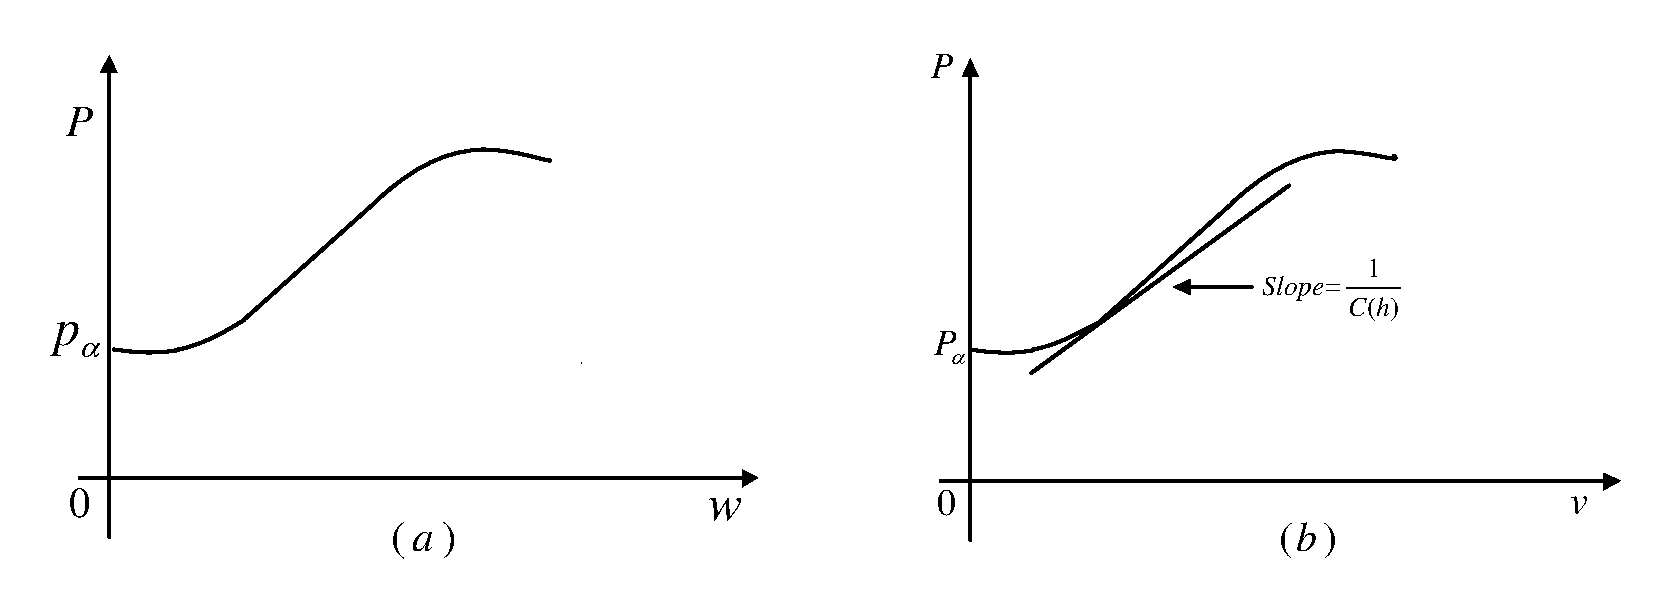
\includegraphics[scale=0.4]{Figura1}
\renewcommand{\figurename}{Fig.}
%\caption{Presi�n en funci�n del volumen y el �rea de un liquido}
\label{Presi�n en funci�n del volumen y el �rea de un liquido}
\end{figure}

Si la tangente para la curva  presión vs volumen es dibujada en algún punto, como se muestra en la figura 1,1 , entonces el recíproco de la pendiente es definido como la capacitancia hidráulica, expresada como \textit{C(h)}.\\

\subsubsection{Ejemplo:}

Considere un vaso formado por un cilindro circular de Radio \textit{R} y Largo \textit{L} que contiene un líquido de densidad \textit{p} en unidades de kilogramo por metro cubico.
Encuentre la capacitancia hidráulica del vaso cuando el cilindro es vertical, como se ve en la figura 2a. También evalúe la capacitancia cuando el cilindro esta sobre uno de sus lados, como se ve en la figura 2b.

\begin{figure}[h]
\centering
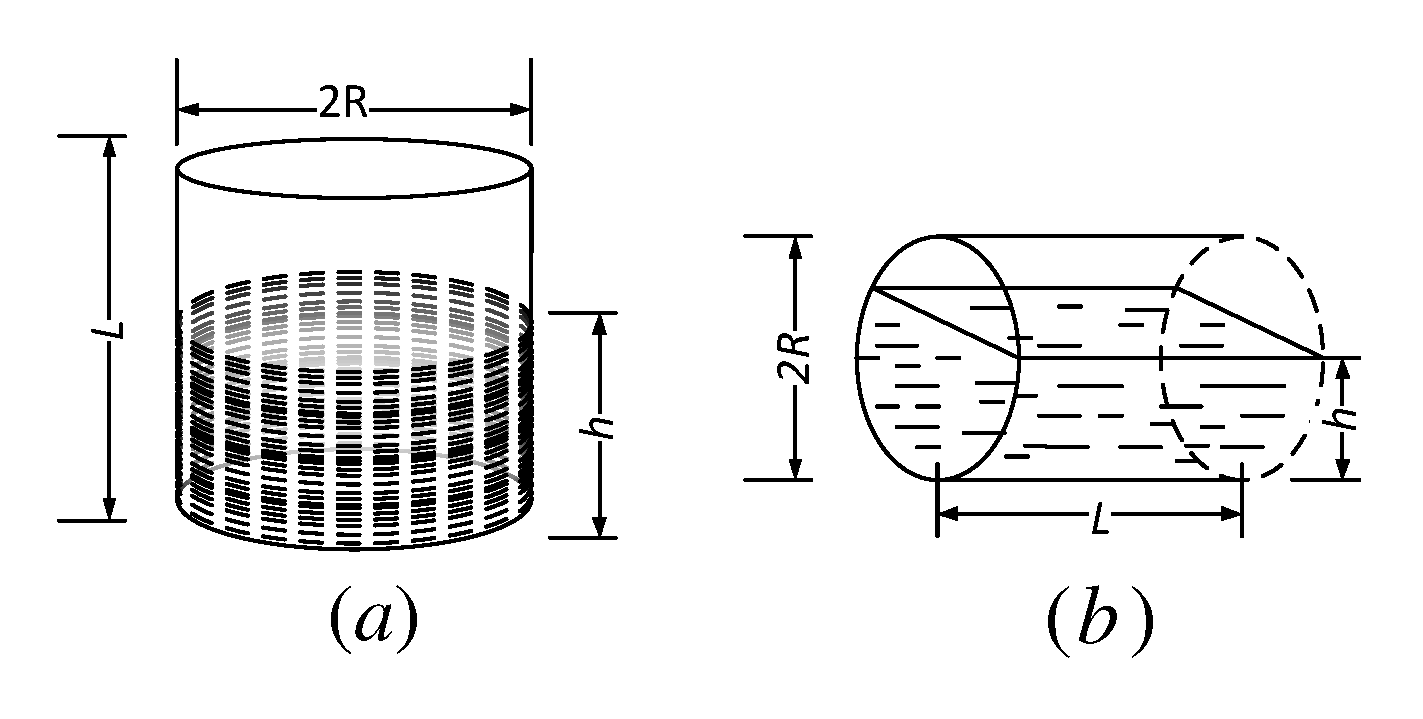
\includegraphics[scale=0.4]{Figura2}
\renewcommand{\figurename}{Fig.}
\caption{Vaso cilíndrico. (a) Vertical. (b) Horizontal.}
\label{Vaso cilíndrico. (a) Cilindro vertical. (b) Cilindro horizontal.}
\end{figure}

\subsubsection{Solución}

Para la configuración en la figura 1,2(a). El área de la sección transversal es ${\pi R^{2}}$ y es independiente de la altura del líquido. Así que podemos usar (1.3), y lacapacitancia hidráulica del recipiente es $C_{a}=\pi\frac{R^{2}}{pg}$ \\

Cuando el recipiente esta sobre uno de sus lados, como se muestra en la figura 2(b), el área de la sección transversal es una función de la altura del liquido h. Puede verificar que el ancho de la superficie del líquido es $2\sqrt{(R^{2})}-(R-h)^{2}$ la cual es cero cuando \textit{h=0} y \textit{h=2R} y tiene el máximo valor de \textit{2R} cuando \textit{h=R}. usando (1.4), encontramos que la capacitancia es:

\begin{equation}
c_{b}=\frac{2L}{pg}\sqrt{R^{2}}-(R-h)^{2}
\label{Ecu 4}
\end{equation}

Como se muestra en la figura 3.

\begin{figure}[h]
\centering
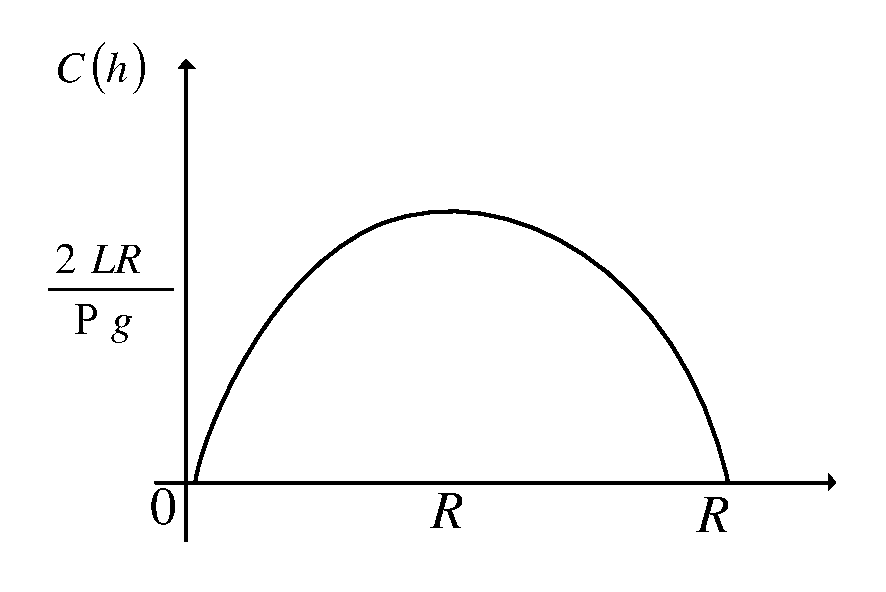
\includegraphics[scale=0.5]{Figura3}
\renewcommand{\figurename}{Fig.}
\caption{Capacitancia del recipiente.}
\label{Capacitancia del recipiente.}
\end{figure}

\subsection{Resistencia}

Como liquido fluye a través de una tubería, allí hay poca presión del líquido a lo largo de la tubería. Del mismo modo ha poca presión si el líquido fluye a través de una válvula o en un orificio. En cambio la presión asociada con el flujo del líquido que resulta la disipación de energía  y usualmente obedece a una relación algebraica no lineal entre la velocidad del flujo $\omega$ la diferencia de presión $\Delta p$. El símbolo de la válvula se muestra en la figura (1.4). Esto también puede ser usado por otros elementos que disipan energía. \\

Un valor positivo de $\omega$ indica que el líquido está fluyendo en la dirección de la flecha; un valor positivo de $\Delta p$ (presión diferencial) indica que la presión en el punto marcado con + es más alta que la presión en el otro punto. La expresión.

\begin{equation}
w=k\sqrt{\Delta p}
\end{equation}

\begin{figure}[h]
\centering
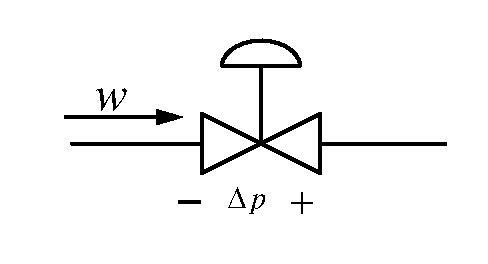
\includegraphics[scale=0.5]{Figura4}
\renewcommand{\figurename}{Fig.}
\caption{simbolo de una válvula hidráulica.}
\label{simbolo de una válvula hidráulica.}
\end{figure}

Describe un orificio y una válvula y es una buena aproximación del flujo turbulento a través de las tuberías. Podemos tratar todas las situaciones de interés para nosotros, usando una ley de un elemento no lineal de la forma de (10). En esta ecuación, k es una constante que depende de las características de la tubería, válvula, u orificio. Una curva típica de la velocidad del flujo contra la presión diferencial como se muestra en la figura 1.5(a).

\begin{figure}[h]
\centering
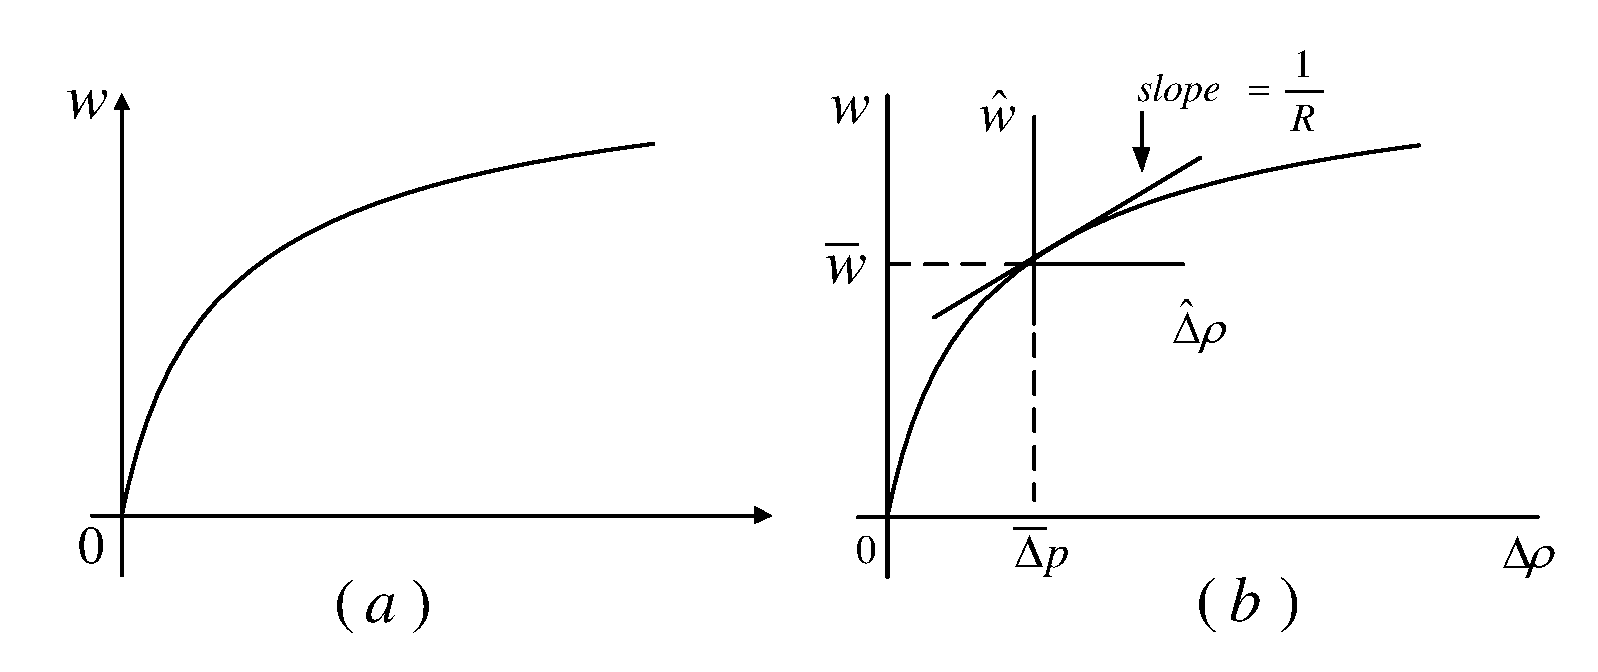
\includegraphics[scale=0.5]{Figura5}
\renewcommand{\figurename}{Fig.}
\caption{(a) velocidad de flujo vs presión diferencial. (b) Interpretación de la resistencia hidráulica.}
\label{(a) velocidad de flujo vs presión diferencial. (b) Interpretación de la resistencia hidráulica.}
\end{figure}

Ya que (10) es una relación no lineal, se debe linealizar alrededor un punto de operación a fin de desarrollar un modelo lineal de un sistema hidráulico.
Si se dibuja la tangente a la curva de w verus $\Delta p$  en el punto de operación, el reciproco de su pendiente es definido como la resistencia hidráulica R. \\

La figura 1.5 (b) ilustra la interpretación geométrica de la resistencia, la cual tiene unidades de newton-segundos por metro.\\

Expandiendo (10) en la serie de Taylor alrededor del punto de operación dado.

\begin{equation}
w=-w+\frac{dw}{d\Delta p}\downarrow -\Delta p (\Delta p -\Delta p - ....)
\end{equation}

La variable incremental $\overline{w}$  y $\overline{\Delta p}$ son definidos por:

\begin{equation}
\widehat{w}=w-\overline{w}
\end{equation}

\begin{equation}
\overline{\Delta p}=\Delta p - \overline{\Delta p} 
\end{equation}

Y el segundo y primer término en la expansión son descartados. Así el modelo incremental se convierte

\begin{equation}
\widehat{w}=\frac{1}{R}-\overline{\Delta p}
\end{equation}

Donde

\begin{equation}
\frac{1}{R}=\frac{dw}{d\Delta p}\downarrow\overline{\Delta p}
\end{equation}

Podemos también expresar la resistencia R en términos de $\overline{\Delta p}$ ó $\overline{w}$llevarlo a la diferenciación requerida usando (10). Específicamente,

\begin{equation}
\frac{1}{R}=\frac{d}{d\Delta p}(k\Delta p_{\frac{1}{2}})\vdots \overline{\Delta p}
\end{equation}

Entonces
\begin{equation}
R=\frac{k}{2\sqrt{\Delta p}}
\end{equation} 
Para expresar la resistencia en términos de $\overline{w}$, se observa de (10) que 
\begin{equation}
\overline{w}=k\sqrt{\overline{\Delta p}}
\end{equation}

Sustituyendo (1.12) en (1.13) dada la ecuación alternativa por resistencia hidráulica como.
\begin{equation}
R=\\frac{2\overline{w}}{k^{2}}
\end{equation}
Ya que los líquidos típicamente fluyen a través de redes compuestas de tuberías, válvulas y orificios, con frecuencia se debe combinar varias relaciones de la forma de (10) en una sola expresión equivalente. Usamos los modelos linealizados en muchos de nuestros análisis de los sistemas hidráulicos, es importante desarrollar reglas para combinar las resistencias de elementos linealizados que estén en configuración serie y paralelo. En el siguiente ejemplo, considere la relación del flujo versus la presión diferencial y la resistencia equivalente para dos válvulas en serie. La situación del flujo paralelo es tratada en uno de los problemas al final del capítulo. \\

\subsubsection{Ejemplo:}

En la figura 5. Se muestra una configuración en serie de dos válvulas a través  de las cuales fluye un líquido con una velocidad w y a través del cual la presión diferencial es ${\Delta p}$, una válvula equivalente se muestra figura 6. Las dos válvulas son.

\begin{figure}[h]
\centering
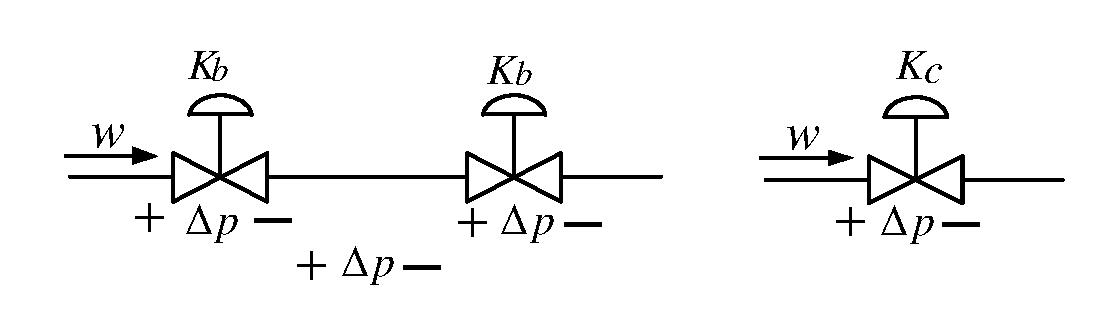
\includegraphics[scale=0.5]{Figura6}
\renewcommand{\figurename}{Fig.}
\caption{Dos válvulas en serie (b). Válvula equivalente.}
\label{Dos válvulas en serie (b). Válvula equivalente.}
\end{figure}

\subsubsection{Solución:}

Ya que las dos válvulas son conectadas en serie, tienen la misma velocidad de flujo $\omega$, y la presión diferencial total es $\Delta p = \Delta_{a}+\Delta_{b}$. Para determinar $k_{c}$, se escribe $\Delta p$ en términos de $\omega$ como:

\begin{equation}
\Delta p= \Delta p_{a}+\Delta p_{b} = \left(\frac{1}{k^{2}_{a}}+\frac{1}{k^{2}_{a}}\right)\omega^{2}
\end{equation} \\

Entonces al resolver para w en términos de $\Delta p$. Después de algunas manipulaciones, se encuentra que:

\begin{equation}
w=\left(\frac{{k_{a}k_{b}}}{\sqrt{{k^{2}}_{a}+{k^{2}}_{b}}} \right)
\end{equation} \\

Comparando (1.16) con (10) se ve que la válvula constante equivalente es

\begin{equation}
k_{c}=\frac{k_{a} k_{b}}{\sqrt{k^{2}}a{k^{2}}b}
\end{equation}

Usando (1.15) para la resistencia  de un modelo linealizado de una válvula equivalente. Se puede escribir:

\begin{equation}
R_{c}\frac{2\overline{\omega}}{k^{2}_{c}}=
2\overline{\omega}(\frac{1}{k^{2}_{a}}+\frac{1}{k^{2}_{b}})
\end{equation} \\

Sin embargo, para aplicar (1.15) a una válvula individual, vemos que estas resistencias son $R_{a}=2\overline{\omega}/k^{2}_{a}$ y $R_{b}=2\overline{\omega}/k^{2}_{b}$ respectivamente. Usando estas expresiones para $R_{a}$ y $R_{b}$, se puede reescribir como:

\begin{equation}
R_{c}=R_{a}+R_{b}
\end{equation}

La cual es idéntica al resultado para un circuito eléctrico lineal. \\

\subsection{Fuentes}

En la mayoría de los sistemas hidráulicos, la fuente de energía es una bomba que deriva su poder de un motor eléctrico. Consideraremos la bomba de tipo centrífuga moviéndose a velocidad constante, que es ampliamente utilizada en procesos químicos. La representación simbólica de una bomba se muestra en la Figura 2.7. Relaciones insumo - producto típicos para una bomba centrífuga siendo conducido a tres velocidades constantes diferentes se muestran en la figura 9. Curvas de la bomba de $\Delta p$ versus $\omega$.\\

%\begin{figure}[h]
%\centering
%\includegraphics[scale=0.5]{}
%\renewcommand{\figurename}{Fig.}
%\caption{Representación simbólica de la bomba.}
%\label{Representación simbólica de la bomba.}
%\end{figure}

%\begin{figure}[h]
%\centering
%\includegraphics[scale=0.5]{}
%\renewcommand{\figurename}{Fig.}
%\caption{Curvas típicas de la bomba centrífuga donde ∆p=p2-p1(a) para tres diferentes velocidades de la bomba (ω1<ω2<ω3). (b) muestra la aproximación lineal.}
%\label{Curvas típicas de la bomba centrífuga donde ∆p=p2-p1(a) para tres diferentes velocidades de la bomba (ω1<ω2<ω3). (b) muestra la aproximación lineal.}
%\end{figure}

Se determinan experimentalmente en condiciones de estado estacionario y son bastante no lineal. Para incluir una bomba está impulsada a una velocidad constante en un modelo dinámico lineal, primero determinamos el punto de funcionamiento de la velocidad de la bomba en particular mediante el cálculo de los valores de \textit{p} y $\omega$. Entonces nos encontramos con la pendiente de la tangente a la curva de la bomba en el punto de trabajo y definimos que sea \textit{-K}, que tiene unidades de newton-segundo por metro. Habiendo Donde está, podemos expresar la diferencia de presión gradual p en términos de la tasa de flujo adicional $\omega$ como:

\begin{equation}
\Delta p=-K\widehat {\omega}
\end{equation}

Donde la constante K es siempre positivo. La solución de la ecuación anterior para $\omega$ produce:

\begin{equation}
\widehat {\omega}=-\frac {1}{K}\widehat {\Delta p}
\end{equation}

Figura 9 (b) Ilustra la relación de la aproximación linealizada a la curva de la bomba no lineal. Podemos escribir la expansión de la series de Taylor para una bomba accionada a una velocidad constante como:

\begin{equation}
\omega =\overline {\omega }+\frac {d\omega }{d\Delta p} \downarrow \frac {\left( \Delta p-\overline {\Delta p}\right)}{\Delta p} +\ldots 
\end{equation}

Donde el coeficiente $\frac {d\omega }{d\Delta p} \downarrow \frac {}{\Delta p}$ esta es la pendiente de la tangente a la curva de $\omega$ versus $\Delta p$, medida en la operación punto, y tiene el valor $-\frac{1}{K}$. Para dejando caer los términos de la segunda y de orden superior en la expansión y el uso de las variables incrementales $\omega$ frente $\widehat{\Delta p}$, obtenemos más la relación lineal de $\widehat {\omega}=-\frac {1}{K}\widehat {\Delta p}$. \\
La manera en cual una constante rápida de la bomba puede estar incorporada entre el modelo dinámico de un sistema hidráulico está ilustrado en el ejemplo 4 en la siguiente sección. \\

\subsection{Modelos Dinamicos de Sistemas Hidraulicos}

En esta sección, se aplican las leyes de los elementos presentados en la sección de sistemas hidráulicos se usan muchas técnicas de análisis  desde el previo capitulo. Vamos a desarrollar y analizar los modelos dinámicos para un solo recipiente con una válvula y una bomba. En cada caso, vamos a derivar el modelo no lineal y luego desarrollar y analizar un modelo linealizado. \\

\subsubsection{Ejemplo 3:}

La Figura 10. Muestra un recipiente que recibe líquido a un caudal $\omega_{i}\left(t\right)$ y pierde  líquido a través de una válvula que obliga la no linealidad de relación flujo contra presión $\omega _{0}=k\sqrt {P_{1}-P_{a}}$. El área de la sección transversal es \textit{A} y la densidad del líquido es  $\rho$. \\
La derivada del modelo no lineal obliga para la presión absoluta $\rho_{1}$ al fondo del recipiente. Luego desarrollar la versión linealizada que es válida en la vecindad de la operación punto, y encontrar la función de trasferencia relacionado la transformación de la entrada incremental $\omega_{i}\left(t\right)$ y la presión incremental $\rho_{1}$. \\

%\begin{figure}[h]
%\centering
%\includegraphics[scale=0.5]{}
%\renewcommand{\figurename}{Fig.}
%\caption{Sistema hidráulico para el ejemplo 3.}
%\label{Sistema hidráulico para el ejemplo 3.}
%\end{figure}

Teniendo desarrollado los modelos de sistemas en forma literal, determinar en forma numérica el punto de operación, la función de transferencia, y la respuesta a un aumento de función al paso del 10\% en el caudal de entrada para los siguientes valores de parámetros:

%\begin{equation}
\begin{center}
$A=2m^{2}$ \\
$\rho=1000\frac {k}{m^{3}}$ \\
$k=5.0\times 10^{-5}\frac {m^{4}}{s}\times N^{\frac {1}{2}}$ \\
$\overline{\omega _{i}}=6.0\times 10^{-3}\frac {m^{3}}{s}$ \\
\end{center}
%\end{equation}

\subsubsection{Solución:}

Tomando la presión p1 como la variable de estado, utilizamos $p=\frac {1}{c}\left[ w_{in}\left( t\right) -W_{out}\left( t\right) \right]$, con $C\left(h\right)$ sustituida por la constante. $C=A/\rho g$, a escribir

\begin{equation}
p=\frac {1}{c}\left[ w_{in}\left( t\right) -W_{out}\left( t\right) \right]
\end{equation}

Luego de reemplazar y sustituir las ecuaciones para el desarrollo del planteamiento del problema se encuentra el sistema de la función de transferencia $H\left( s\right) =p_{1}\left( s\right) /w_{i}\left( s\right)$ es

\begin{equation}
H\left( s\right) =\frac {\frac {1}{C}}{s+\frac {1}{RC}}
\end{equation}

Cual tiene un solo polo en S= -1RC. Para el valor del parámetro especificado, el punto de operación dada se reduce a

\begin{equation}
P_{1}=1.013\times 10^{5}+\left( \frac {6.0\times 10^{-3}}{5.0\times 10^{-5}}\right) ^{2}=1.157\times 10^{5}\frac {N}{m^{2}}
\end{equation}

La altura nominal del líquido es

\begin{equation}
h=\frac {1.440\times 10^{4}}{1000\times 9.807}=1.468m
\end{equation}

El valor numérico de la resistencia hidráulica y capacitancia son, respectivamente,

\begin{equation}
R=\frac {2\times 60\times 10^{-3}}{\left( 50\times 10^{-5}\right) ^{2}}=4.80\times 10^{6}N\times S/m^{5}
\end{equation}

\begin{equation}
C=\frac {20}{1000\times 9.807}=2.039\times 10^{-4}m^{5}/N
\end{equation}

Sustituyendo este valor de R y C entre la ecuación anterior de la función de transferencia, se puede obtener la forma numérica  de la función de transferencia como

\begin{equation}
H\left( s\right) =\frac {4904}{s+1.0216\times 10^{-3}}
\end{equation} \\

Si $\omega_{i}(s)$ es originalmente igual a este valor nominal de $\overline {w}_{i}=6.0\times 10^{-3}m^{3}/s$ y sufre un 10\% aumento paso a la función, luego $w_{i}\left( t\right) =\left[ 0.60\times 10^{-3}\right] U\left( t\right) \frac {m^{3}}{s}$ y $w_{i}\left( s\right) =\left[ 0.60\times 10^{-3}\right] \left( \frac {1}{s}\right)$. Tenemos.

\begin{equation}
P_{1}\left( s\right) =\frac {4904\times 0.60\times 10^{-3}}{s\left( s+1.0216\times 10^{-3}\right) }
=\frac {2.942}{s\left( s+1.0216\times 10^{3}\right) }
\end{equation}

Del teorema del valor final, el estado estacionario de p1 es p1(s) evaluado en s=0, a saber

\begin{equation}
\lim _{t\rightarrow \infty }P_{1}\left( t\right) =\frac {2942}{1.0216\times 10^{-3}}=2880N/m^{2}
\end{equation}

La constante de tiempo del modelo linealizado es $\tau = RC$ , cual se convierte en 

\begin{equation}
\tau =\left( 4.80\times 10^{6}\right) \left( 2.039\times 10^{-4}\right) =978.7s
\end{equation}

Que es un poco más de 16 minutos. Tenemos la respuesta que la  presión incremental es

\begin{equation}
P_{1}=2888\left( 1-\in \right) \ldots falta\ldots
\end{equation}

El cambio en el nivel incremental es p1/p, cual se convierte en 

\begin{equation}
h=0.2937\left( 1-\in \right) \ldots falta\ldots 
\end{equation}

A obtener la respuesta de la presión del caudal y el nivel de líquido, nos limitamos a añadir los valores nominales $p_{1}=1.157\times 10^{5}\frac {N}{m^{2}}$ y $h=1.468m$  de las variables incrementales. Es interesante observar que a causa de la válvula no lineal, el aumento del 10\% en los resultados de la velocidad de flujo en un aumento del 20\% tanto en la presión manométrica p1-pa y la altura h. \\

\subsubsection{Ejemplo 4:}

Encontrar el modelo linealizado del sistema hidráulico mostrado en la Figura 11 (a) que consiste en una bomba centrífuga de velocidad constante la alimentación de un recipiente desde el cual fluye líquido a través de una tubería y válvula de obedecer a la relación $\omega _{0}=k\sqrt {P_{1}}-P_{a}$. La característica de la bomba de la velocidad W de la bomba especificada se muestra en la figura 12.11 (b). \\

\subsubsection{Solución:}

La condición equilibrada para el sistema corresponde a 

\begin{equation}
\omega _{i}=\omega _{0}
\end{equation}

Donde $\omega_{i}$ y $\Delta p=p_{1}-p_{a}$ debe ser uno de los puntos de la curva de la bomba en la Figura 11 (b), y donde $\omega_{o}$ obedece a la relación de flujo no lineal.

\begin{equation}
\omega_{o}=K\sqrt{\Delta p}
\end{equation}

Para determinar el punto de trabajo, nos encontramos con la solución de  $\omega_{i}=\omega_{o}$  gráficamente trazando la característica de la válvula  $\omega_{o}=K\sqrt{\Delta p}$  en la curva de la bomba. Hacer esto dada la Figura 12 (a), en el que el punto de trabajo es la intersección de la curva de la válvula y la curva de la bomba, designado como punto A en la figura, una vez que hemos localizado el punto de operación, podemos trazar la tangente a la curva de la bomba como se muestra en la figura 12 (b) y determinar su pendiente -K gráficamente. \\

%\begin{figure}[h]
%\centering
%\includegraphics[scale=0.5]{}
%\renewcommand{\figurename}{Fig.}
%\caption{(a) sistema para el Ejemplo 4. (b) Curva de la bomba}
%\label{(a) sistema para el Ejemplo 4. (b) Curva de la bomba}
%\end{figure}

%\begin{figure}[h]
%\centering
%\includegraphics[scale=0.5]{}
%\renewcommand{\figurename}{Fig.}
%\caption{(a) Curvas de bombas y válvulas combinadas del Ejemplo 4. (b) curva de la bomba con la aproximación lineal.}
%\label{(a) Curvas de bombas y válvulas combinadas del Ejemplo 4. (b) curva de la bomba con la aproximación lineal.}
%\end{figure}

Después de esta etapa preliminar, podemos utilizar $p_{1}=\frac{1}{c} \left(\omega_{i}-\omega_{o}\right)$ para escribir el modelo desde el sistema como:

\begin{equation}
p_{1}=\frac{1}{c} \left(\omega_{i}-\omega_{o}\right)
\end{equation}

dDonde, de $\widehat {\omega }=\frac {1}{R}\widehat {\Delta P}$, el caudal aproximado a través de la válvula es 

\begin{equation}
\omega _{0}=\overline {\omega _{0}}+\frac {1}{R}\widehat {\Delta p}
\end{equation}

Y donde, de $\widehat {\omega }=-\frac {1}{K}\widehat {\Delta p}$, el caudal aproximado a través de la bomba es

\begin{equation}
\omega _{i}=\overline {\omega }_{i}-\frac {1}{k}\widehat {\Delta \rho }
\end{equation}

Sustituyendo las ecuaciones anteriores entre el modelo del sistema, usando $p_{1}=\widehat {p_{1}}$ y $\omega_{i}=\omega_{o}$, y nada que $\widehat {\Delta p}=p_{1}$ porque $p_{a}$ es constante, se encuentra el modelo incremental es 

\begin{equation}
P_{1}=\frac {1}{c}\left( -\frac {1}{k}-\frac {1}{R}\right) P_{1}
\end{equation}

Cual se puede escribir como homogéneo de primer orden de la ecuación diferencial.

\begin{equation}
P_{1}+\frac {1}{c}\left( \frac {1}{k}+\frac {1}{R}\right) P_{1}=0
\end{equation}

La ecuación anterior indica que la magnitud de la pendiente de la curva sobre la bomba en el punto de operación  está entre la ecuación exactamente igual como la resistencia asociada con la válvula. 

Luego, si se evalúa la resistencia equivalente $R_{eq}$ se acuerda

\begin{equation}
R_{eq}=\frac {RK}{R+K}
\end{equation}

La cual fue derivada por un recipiente y una sola válvula, excepto por la ausencia de un caudal de entrada. \\

\subsubsection{Ejemplo 5:}

Las válvulas en el sistema hidráulico se muestra en la Figura 13 obedece el flujo de presión con la relación $\omega _{1}=K_{1}\sqrt {p_{1}}-P_{2}$ y $\omega _{2}=K_{2}\sqrt {p_{2}}-P_{a}$. La presión atmosférica es $p_{a}$, y las capacitancias de los tanques son $C_{1}$ y $C_{2}$. \\
Encuentre las ecuaciones que determine el punto de operación, y muestra como la curva de bomba es usada entonces. Un modelo derivado linealizado que es válido sobre el punto de operación. \\

\subsubsection{Solución:}

Porque la bomba y los dos tanques son en serie que equilibra las condiciones, se define el punto de operación para los tres caudales sean iguales $\omega_{p}$, $\omega_{1}$ y $\omega_{2}$.

%\begin{figure}[h]
%\centering
%\includegraphics[scale=0.5]{}
%\renewcommand{\figurename}{Fig.}
%\caption{Sistema hidráulico con dos tanques considerando el Ejemplo 5.}
%\label{Sistema hidráulico con dos tanques considerando el Ejemplo 5.}
%\end{figure}

Los caudales a través de dos válvulas son dados por

\begin{equation}
\omega _{1}=K_{1}\sqrt {p_{1}}-P_{2}
\end{equation}

\begin{equation}
\omega _{2}=K_{2}\sqrt {p_{2}}-P_{a}
\end{equation}


El caudal $\omega_{p}$ que pasa a través de la bomba y la presión diferencial $\Delta p_{1}=p_{1}-p_{a}$ corresponde más a un punto sobre la curva de la bomba.

\begin{equation}
\omega _{p}=k_{eq}\sqrt {\Delta p_{1}}
\end{equation}

Donde,

\begin{equation}
K_{eq}=\frac {K_{1}K_{2}}{\sqrt {k^{2}_{1}}+\left( k_{2}\right) ^{2}}
\end{equation}

Graficando la ecuación anterior sobre la curva de la bomba como se muestra en la Figura 12(a) siendo las válvulas de $\Delta p_{1}$ y $\omega_{p}$, de la cual se puede encontrar otro valor nominal. \\
Con esta información, se puede desarrollar el modelo incremental. Usando $p=\frac {1}{c\left( n\right) }\left[ \omega _{in}\left( t\right) -\omega _{out}\left( t\right) \right] $,  $\omega =\frac {1}{R}\Delta p$, y $\omega =-\frac {1}{K}\Delta p$, se puede escribir el par de ecuaciones diferenciales.

\begin{equation}
p_{1}=\frac {1}{C_{1}}\left[ -\frac {1}{K}P_{1}-\frac {1}{R_{1}}\left( P_{1}-P_{2}\right) \right] 
\end{equation}

\begin{equation}
p_{1}=\frac {1}{C_{2}}\left[ -\frac {1}{R_{1}}\left( P_{1}-P_{2}\right) -\frac {1}{R_{2}}P_{2}\right] 
\end{equation}

Donde las resistencias de las válvulas son dadas por $R_{1}=\frac {2\omega _{1}}{\left( k_{1}\right) ^{2}}$ y $R_{2}=\frac {2\omega _{2}}{\left( k_{2}\right) ^{2}}$, y donde –K es la pendiente de la curva de la bomba en el punto de operación. Como se indica en las ecuaciones anteriores, el modelo incremental no tiene entrada y por lo tanto puede responder solo a una condición inicial que no sea cero, que es $p_{1}(0)$ diferente de cero y/o $p_{2}$ diferente de cero. \\
En la práctica, puede haber corrientes líquidas adicionales que entran ya sea buque, o la velocidad de la bomba puede ser cambiada. También es posible para cualquiera de las dos válvulas que se abren o se cierran ligeramente. Tal cambio modificaría la respectiva resistencia hidráulica. \\
En la ausencia de una entrada, se puede transformar la ecuación anterior a encontrar la transformada de Laplace de la respuesta cero de entrada. Haciendo esto, se encuentra que después se ve:

\begin{equation}
\left[ C_{1}s+\left( \frac {1}{k}+\frac {1}{R_{1}}\right) \right] P_{1}\left( s\right) =\frac {1}{R_{1}}P_{2}\left( s\right) +C_{1}P_{1}\left( 0\right) 
\end{equation}

\begin{equation}
\left[ C_{1}s+\left( \frac {1}{R_{1}}+\frac {1}{R_{2}}\right) \right] P_{2}\left( s\right) =\frac {1}{R_{1}}P_{1}\left( s\right) +C_{2}P_{2}\left( 0\right) 
\end{equation}

Se puede encontrar cualquiera de las dos presiones $p_{1}$ o $p_{2}$ para combinarlas en estas dos ecuaciones entre una singular transformada. La correspondiente transformada inversa producirá la respuesta de entrada cero en términos $p_{1}$ y $p_{2}$. El denominador de cualquiera de las dos $p_{1}$ y $p_{2}$ estará la característica del polinomio del sistema, el cual, como se puede verificar, es:

\begin{equation}
s^{2}+\left[ \frac {1}{C_{2}}\left( \frac {1}{K}+\frac {1}{R_{1}}\right) +\frac {1}{C_{2}}\left( \frac {1}{R_{1}}+\frac {1}{R_{2}}\right) \right] s+\frac {1}{C_{1}C_{2}}\left( \frac {1}{kR_{1}}+\frac {1}{KR_{2}}+\frac {1}{R_{1}R_{2}}\right) 
\end{equation}














\newpage



% ==============================================================================================
%										SECCIÓN MODELAMIENTO
% ==============================================================================================


\section{Modelamiento}

\begin{equation}
A\frac {dh\left( t\right) }{dt}=q_{i}-q_{o}
\end{equation}

Teniendo en cuenta 	que

\begin{equation}
q_{o}=\frac{h}{R}
\end{equation}

Ya que el nivel del tanque es la variable monitoreada se convierte en derivable.\\
Se reemplaza (1) en (2)

\begin{equation}
A\frac {dh\left( t\right) }{dt}=q_{i}-\frac {h}{R}
\end{equation}

Se tiene en cuenta que \textit{h}, $Q_{in}$ son variables dependientes de \textit{(t)}

\begin{equation}
\frac {dh\left( t\right) }{dt}=\frac {q_{i}-\frac {h}{R}}{A}
\end{equation}

Separando variables derivables y no derivables

\begin{equation}
\frac {dh\left( t\right) }{dt}=\frac {Rq_{i}-h}{AR}
\end{equation}

Evaluando en estado estable, $t=0$

\begin{equation}
\frac {d\overline {h\left( 0\right) }}{dt}=\frac {R\overline {q_{i}\left( 0\right) }-\overline {h\left( o\right) }}{AR}
\end{equation}

Operando (resta) (4)-(5) de las variables

%\begin{equation}
%\end{equation}

\begin{equation}
ARd\frac {\left[ h\left( t\right) -\overline {h\left( 0\right) }\right] }{dt}=R\left[ q_{i}\left( t\right) -\overline {q_{i}\left( 0\right) }\right] -\left[ h\left( t\right) -\overline {h\left( 0\right) }\right]
\end{equation}

Realizando cambio de variable

\begin{equation}
Q_{in}=q_{i}\left( t\right) -\overline {q_{i}\left( 0\right) }
\end{equation}

\begin{equation}
H=h\left( t\right) -\overline {h\left( 0\right) }
\end{equation}

\begin{equation}
A\frac {RdH}{dt}=RQ_{in}\left( t\right) -H\left( t\right)
\end{equation}

Se separan las variables de nivel a un lado de la ecuación

\begin{equation}
A\frac {RdH}{dt}+H\left( t\right) =RQ_{in}\left( t\right)
\end{equation}

Realizando segundo cambio de variable en la ecuación 7 \\

\begin{center}
$\tau =AR$ \\
$K=R$
\end{center}

\begin{equation}
\frac {\tau dH}{dt}+H\left( t\right) =KQ_{in}\left( t\right)
\end{equation}

Se aplica transformada de Laplace para derivada de primer orden en la ecuación 8

\begin{equation}
\tau sH\left( s\right) +H\left( s\right) =kQ_{in}\left( s\right)
\end{equation}

Se factorizan terminos de altura \textit{H}

\begin{equation}
H\left( s\right) \left[ \tau s+1\right] =kQ_{in}\left( s\right)
\end{equation}

$H(s)$ equivale a la salida del sistema y $Q_{in}(s)$ a la entrada ya que el modelo de función de transferencia es $G=out/in$, se tiene que

\begin{equation}
\frac {H\left( s\right) }{Q_{in}\left( s\right) }=\frac {k}{\tau s+1}
\end{equation}

(Modelo de función de transferencia de primer orden) \\

Para realizar el modelo especifico del tanque, es necesario realizar el cambio de variable inverso a la ecuación (8) aplicando la ecuación (11)

\begin{equation}
\frac {H\left( s\right) }{Qin\left( s\right) }=\frac {R}{AR+1}
\end{equation}




\newpage



% ==============================================================================================
%										SECCIÓN LINEALIZACIÓN
% ==============================================================================================

\section{Linealización}

Un sistema no lineal se define siempre y cuando no se aplique el principio de superposición, es decir, la respuesta a dos entradas no puede calcularse tomando cada una de ellas independientemente y luego sumarlas, debido a esto se usa la linealización.\\

%\begin{figure}[h]
%\centering
%\includegraphics[scale=0.5]{}
%\renewcommand{\figurename}{Fig.}
%\caption{Principio de Superposición.}
%\label{Principio de Superposición.}
%\end{figure}

La linealización es un método matemático por el cual se aproxima un sistema no lineal a uno más sencillo de analizar con una solución general del comportamiento del proceso y alrededor de un punto de operación cualquiera \textit{(xs,us)}.\\

Así pues, una función lineal es una aproximación de la función original, que se representa trazando una línea tangente al punto de operación, que se puede interpretar con la siguiente figura:\\

%\begin{figure}[h]
%\centering
%\includegraphics[scale=0.5]{}
%\renewcommand{\figurename}{Fig.}
%\caption{Punto de Operación de una función linealizada.}
%\label{Punto de Operación de una función linealizada.}
%\end{figure}

De este modo, la función linealizada solo es válida en el interior de la región representada por el círculo alrededor del punto negro en la figura 2.

%\begin{equation}
\begin{center}
	$f\left( x,u\right)=0$ \\
	$f\left( x_{s},u_{s}\right) =0$ \\
	$f\left( x,u\right) = f\left( x_{s},u_{s}\right) +\frac {\partial f}{\partial u}\left( x-x_{s}\right) +\frac {\partial f}{\partial u}\left( u+u_{s}\right) +\ldots$ \\
	$\frac {\partial f}{\partial x}\Delta x+\frac {\partial f}{\partial u}\Delta u=0$
\end{center}
%\end{equation}

\subsection{Características sistemas linealizados}

\begin{enumerate}
\item La ecuación linealizada no es única, depende del punto alrededor del cual se haya linealizado.
\item Las variables de la ecuación linealizada están dadas por incrementos con referencia al punto de operación.
\item Es más sencillo linealizar las ecuaciones término a término.
\item Diferencias de comportamiento entre el modelo linealizado y el real
\item Forma de la función a linealizar.
\item Las diferencias aumentan al alejarse del punto de equilibrio 
\end{enumerate}

\subsection{Serie de Taylor}

Para linealizar un sistema existen varios métodos tales como logaritmación, cambio de variable, series de Taylor y mínimos cuadrados, sin embargo uno muy común y el cual se utilizara en este caso son las series de Taylor, que se expresan como una suma infinita de los términos de una función.\\

Una función infinitamente derivable en un intervalo puede representarse como un polinomio a partir de sus derivadas evaluadas en un punto “a” de dicho intervalo.

%\begin{equation}
\begin{center}
	$f\left( x\right) =\sum ^{\infty }_{n=0}f^{n}\left( a\right) \frac {\left( x-a\right) ^{n}}{n!}$
\end{center}
%end{equation}

\subsubsection{Ejemplo 1:}

%\begin{equation}
\begin{center}
	$f^{0}\left( x\right) =f\left( x\right) =e^{x}$
\end{center}
%\end{equation}

\begin{enumerate}

\item Definir las derivadas de la función.
	%\begin{equation}
	\begin{center}
		$f^{1}\left( x\right) =f'\left( x\right) =e^{x}$\\
		$f^{2}\left( x\right) =f''\left( x\right) =e^{x}$\\
		$f^{3}\left( x\right) =f'''\left( x\right) =e^{x}$
	\end{center}
	%\end{equation}
\item Definir un punto de operación “a”.
	\begin{center} a=0 \end{center}
\item Definir los valores para “n” desde 0 hasta 3, hay que tener en cuenta que “n” puede llegar a valer $\infty$, sin embargo, entre mayor sea, más pequeño es el valor del termino y por tanto es despreciable para el resultado final de la ecuación. El valor de “n” también depende del número de derivaciones que pueda llegar a tener una ecuación determinada.\\

	n=0
	%\begin{equation}
	\begin{center}
		$f^{0}\left( 0\right) \frac {\left( x-0\right) ^{0}}{0!}=f^{0}\left( 0\right) \frac {1}{1}=f^{0}\left( 0\right)$\\
		$f^{0}\left( 0\right) =f\left( 0\right) =e^{0}=1$ \\
		\textit{ Primer término de la serie }\\
	\end{center}
	%\end{equation}
	
	n=1
	%\begin{equation}
	\begin{center}
		$f^{1}\left( 0\right) \frac {\left( x-0\right) ^{1}}{1!}=f^{1}\left( 0\right) \frac {x}{1}=x\cdot f^{1}\left( 0\right)$\\
		$x\cdot f^{1}\left( 0\right) =x\cdot f'\left( 0\right) =x\cdot e^{0}=x$\\
		\textit{ Segundo término de la serie }\\
	\end{center}
	%\end{equation}
	
	n=2
	%\begin{equation}
	\begin{center}
		$f^{2}\left( 0\right) \frac {\left( x-0\right) ^{2}}{2!}=f^{2}\left( 0\right) \frac {x^{2}}{2}=\frac {x^{2}\cdot f^{2}\left( 0\right) }{2}$\\
		$\frac {x^{2}\cdot f^{2}\left( 0\right) }{2}=\frac {x^{2}\cdot f''\left( 0\right) }{2}=\frac {x^{2}}{2}\cdot e^{0}=\frac {x^{2}}{2}$\\
		\textit{ Tercer término de la serie }\\
	\end{center}
	%\end{equation}
	
	n=3
	%\begin{equation}
	\begin{center}
		$f^{3}\left( 0\right) \frac {\left( x-0\right) ^{3}}{3!}=f^{3}\left( 0\right) \frac {x^{3}}{6}=\frac {x^{3}\cdot f^{2}\left( 0\right) }{6}$\\
		$\frac {x^{3}\cdot f^{3}\left( 0\right) }{6}=\frac {x^{3}\cdot f'''\left( 0\right) }{6}=\frac {x^{3}}{6}\cdot e^{0}=\frac {x^{3}}{6}$\\
		\textit{ Cuarto término de la serie }\\
	\end{center}
	%\end{equation}
	
\item La serie de Taylor para $f(x)=e^{x}$ es:
	%\begin{equation}
	\begin{center} $1+x+\frac {x^{2}}{2}+\frac {x^{3}}{6}+\ldots$ \end{center}
	%\end{equation}
\end{enumerate}

\subsubsection{Ejemplo 2:}

Considere el siguiente sistema:

Variables de desviación

%\begin{equation}
\begin{center}
	$\Delta h=h-h_{0}$\\
	$\Delta q=q-q_{0}$\\
	$A\frac {dh}{dt}-q+k\sqrt {h}=0$\\
\end{center}
%\end{equation}




\newpage



% ==============================================================================================
%										SECCIÓN IDENTIFICACIÓN
% ==============================================================================================

\section{Identificación}
%\chapter{Identificación}


\newpage



% ==============================================================================================
%											SECCIÓN CONTROL
% ==============================================================================================

\section{Control}

\subsection{Uso de SISOTOOL Para diseño de controles}

Sisotool es una poderosa herramienta de MATLAB que facilita en gran medida el diseño de controles. En \textit{sisotool} se trabaja de forma gráfica, usando el  método del $LGR$ (lugar geométrico de las raíces). \textit{Sisotool} puede mostrar en tiempo real las variaciones  de la respuesta del sistema generadas por los cambio que el usuario realice en el $LGR$, y es esto lo que lo hace tan practico para el diseño de controles. Para ejecutar \textit{sisotool} basta con llamarlo desde la línea de comando de MATLAB  escribiendo \textit{“sisotool”}. \\

Lo primero que se debe hacer antes de empezar a utilizar \textit{sisotool} es definir la planta a controlar. Para esto se debe tener un modelo de la planta, es decir su función de transferencia. Sino se tiene el modelo de la planta es imposible utilizar \textit{sisotool} para el diseño de un controlador. \\

una vez se tiene el modelo de la planta se procede a realizar su definición en MATLAB, esta se hace con la función \textit{"tf"}. Por ejemplo, a continuación se procede a definir la siguiente planta: \\

\begin{figure}[h]
\centering
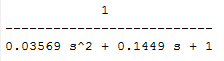
\includegraphics[scale=1.0]{FuncionPlanta}
\renewcommand{\figurename}{Fig.}
\caption{Función de transferencia de la Planta.}
\label{Función de transferencia de la Planta.}
\end{figure}

Primero se debe definir un vector con los coeficientes del numerador y otro con los coeficientes del denominador. Los vectores deben empezar por el coeficiente que multiplica a \textit{s} con mayor exponente hasta llegar al coeficiente que multiplica a \textit{s} con potencia cero, es decir el que no multiplica a ningún \textit{s}. Si al polinomio de \textit{s} le hace falta alguna potencia de \textit{s} quiere decir que el coeficiente para esa potencia de \textit{s} es igual a cero. Por ejemplo, el vector de coeficientes para el polinomio $s^{4}+2s^{2}+s$ debe ser $[1 0 2 1 0]$.  Entonces la definición de la planta mencionada quedaría como sigue: \\

\begin{center}
$num=[1];$ \\
$den=[0.03569  0.1449  1];$ \\
$G=tf(num,den);$ \\
\end{center}

Al ejecutar estos comandos se crea en el \textit{Workspace} de Matlab una función de transferencia de la planta con el nombre \textit{"G"}, debido a que \textit{G} fue el nombre que le fua easignado al ejecutar la función \textit{"tf"}. Ahora se procede a ejecutar \textit{sisotool}, si no se había realizado con anterioridad. Ejecutamos \textit{"sisotool"} en la linea de comandos de MATLAB y se abriran dos ventanas. Una se llama \textit{"Control and Estimation Tool Manager"} y la otra \textit{"SISO design for SISO Design Task"}. A continuación se muestran imágenes de las ventanas emergentes. Si no se abren ventanas parecidas a estas, probablemente este utilizando una versión antigua de \textit{Sisotool}. \\

\begin{figure}[h]
\centering
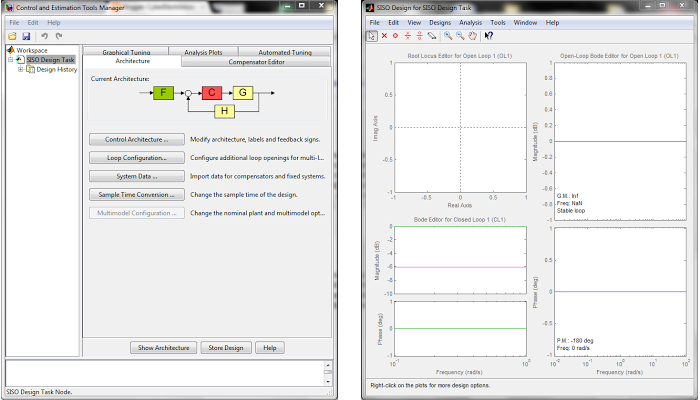
\includegraphics[scale=0.5]{Ventana1}
\renewcommand{\figurename}{Fig.}
\caption{(a) Control and Estimation Tool Manager. (b) SISO design for SISO Design Task.}
\label{Control and Estimation Tool Manager.}
\end{figure}

En \textit{“Control and Estimation Tool Manager”} se escoge la arquitectura de control a utilizar. En la pestaña \textit{“Architecture”}, al dar clic en el botón \textit{“Control Achitecture”} se despliega una ventana que muestra una lista de las arquitecturas disponibles. Para este ejemplo se ha seleccionado la primera de la lista, que se muestra en la \textit{Figura 2.8}. \\

\begin{figure}[h]
\centering
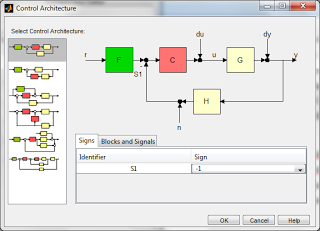
\includegraphics[scale=0.7]{Ventana2}
\renewcommand{\figurename}{Fig.}
\caption{Control Architecture.}
\label{Control Architecture.}
\end{figure}

Después de seleccionar la arquitectura, se importa la función de transferencia de $G(s)$ desde la ventana \textit{“SISO Desing for SISO Desing Task”},  con la opción \textit{“importar”} del menú \textit{“File”}. AL dar clic en \textit{“importar”} Se despliega una ventana en donde se muestra una lista de los sistemas de la arquitectura seleccionada, en este caso  $G$, $H$, $C$ y $F$ que por defecto tienen el valor de \textit{"1"}. La imagen de esta ventana se muestra en la \textit{Fig. 2.9}. \\

\begin{figure}[h]
\centering
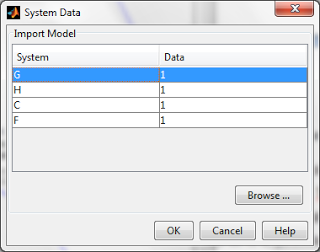
\includegraphics[scale=0.7]{Ventana3}
\renewcommand{\figurename}{Fig.}
\caption{System Data.}
\label{System Data.}
\end{figure}

Se selecciona \textit{“G”} que corresponde a la planta y se presiona \textit{“Browser”}. Entonces aparece otra ventana que muestra una lista de las funciones de transferencia que se encuentran en el \textit{WorkSpace} y en donde debe estar la función \textit{“G”} definida anteriormente y que corresponde a nuestra planta. La imagen de la nueva ventana es la \textit{Fig. 2.10}. \\

\begin{figure}[h]
\centering
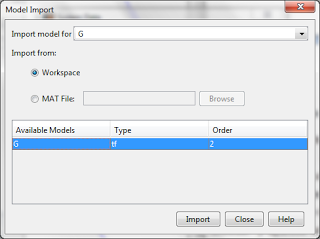
\includegraphics[scale=0.7]{Ventana4}
\renewcommand{\figurename}{Fig.}
\caption{Model Import.}
\label{Model Import.}
\end{figure}

Ahora se selecciona la planta, es decir \textit{“G”}. Se presiona \textit{“import”}, se cierra esta ventana y por último se presiona \textit{“OK”} en la ventana anterior. Habiendo hecho esto, las gráficas de la ventana \textit{"SISO design for SISO Design Task"} debieron modificarse, dicha ventana debe quedar como se observa en la \textit{Fig. 2.11}. \\

\begin{figure}[h]
\centering
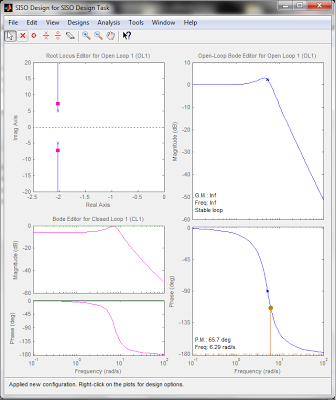
\includegraphics[scale=0.7]{Ventana5}
\renewcommand{\figurename}{Fig.}
\caption{SISO design for SISO Design Task.}
\label{SISO design for SISO Design Task.}
\end{figure}

En la parte superior izquierda de esta ventana se observa la gráfica del $LGR$. Las lineas azules de esta gráfica son el $LGR$ y los puntos rosados representan   la posición actual de los polos del sistema a lazo cerrado. En la arquitectura que se escogió y en general \textit{"C"} es el compensador, y es este sobre el que se enfoca el diseño. Es decir, se necesita encontrar un compensador que haga que el sistema funcione como se desea. \\

Uno de los parametros principales como punto de partida es la definición de la meta a lograr con el control. Para este ejemplo se busca mejorar la respuesta transitoria del sistema, es decir la respuesta del sistema a un escalón. En primer lugar debemos conocer la respuesta del sistema a lazo abierto, es decir de la planta. Para esto utilizamos la herramienta \textit{“Response to step command”} de \textit{sisotool} que se encuentra en el menú \textit{"Analysis"} de la ventana  \textit{"SISO design for SISO Design Task"}. Al ejecutarlo se abre una ventana en la cual aparecen dos gráficas. Esta ventana se muestra en la \textit{Fig. 2.12}. \\

\begin{figure}[h]
\centering
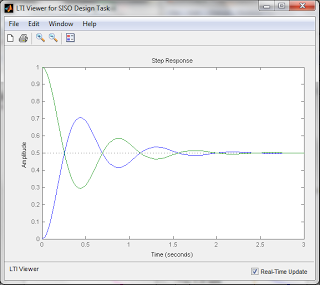
\includegraphics[scale=0.7]{Ventana6}
\renewcommand{\figurename}{Fig.}
\caption{LTI Viewer for SISO Design Task.}
\label{LTI Viewer for SISO Design Task.}
\end{figure}

La gráfica de color Azul es la respuesta del sistema a lazo cerrado y la gráfica de color verde es la señal de salida del compensador. Para ver la respuesta de la planta se da un clic derecho sobre la gráfica, se selecciona \textit{"Systems"} y después \textit{"PlantG"}. Así como se muestra en la \textit{Fig. 2.13}. \\

\begin{figure}[h]
\centering
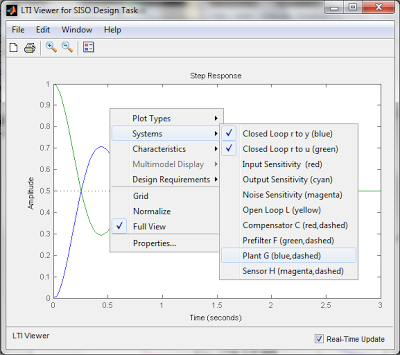
\includegraphics[scale=0.6]{Ventana7}
\renewcommand{\figurename}{Fig.}
\caption{LTI Viewer for SISO Design Task.}
\label{LTI Viewer for SISO Design Task.}
\end{figure}

Entonces aparece una tercera gráfica, de color azul pero con una linea discontinua. Esta es la respuesta transitoria de nuestra planta y nos sirve como referencia para determinar si la respuesta transitoria del sistema a lazo cerrado ha mejorado o no. \\

\begin{figure}[h]
\centering
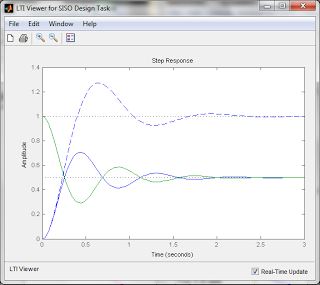
\includegraphics[scale=0.7]{Ventana8}
\renewcommand{\figurename}{Fig.}
\caption{LTI Viewer for SISO Design Task.}
\label{LTI Viewer for SISO Design Task.}
\end{figure}

Ahora regresamos a la ventana de trabajo, la ventana en donde aparece el $LGR$. Los puntos rosados en el $LGR$ representan la posición actual de los polos del sistema a laso cerrado. Estos puntos solo pueden estar sobre la linea de color azul, es decir sobre el $LGR$. Por lo que si se desea poner los polos en una determinada posición, el $LGR$ debe pasar por ahí. Lo anterior es muy importante, mas adelante se explica el por que. \\

Ahora se procede a determinar en donde se deben poner los polos para obtener la respuesta deseada. Pues bien, para solucionarlo \textit{Sisotool} ofrece la posibilidad de incluir algunos requerimientos de diseño en la gráfica del $LGR$. Esto quiero decir que al especificar los requerimientos del diseño, \textit{sisotool} traza una gráfica sobre el $LGR$ que proporciona una idea de donde deben estar los polos para que el sistema funcione como se desea. A continuación se procede a definir que polos deben estar en los puntos que indica \textit{sisotool}, deben ser los polos dominantes. \\

Los polos dominantes son aquellos que más intervienen en la respuesta de un sistema. Aunque la respuesta de un sistema no está completamente determinada por los polos dominantes, puede hallarse una muy buena aproximación de esta hallando la respuesta solo a partir de la contribución de estos polos. Como regla general se toman como polos dominantes aquellos que están más cerca al origen, pues son los que más influyen en la respuesta. \\

Ahora se agregan los requerimientos del diseño. Para este ejemplo se agregan dos requerimientos de diseño: el tiempo de asentamiento o \textit{"Settling time"} y el porcentaje de sobrepaso o \textit{"Percent Overshoot"}. Para agregar un nuevo requerimiento de diseño se da un clic derecho sobre la gráfica del $LGR$ y se selecciona \textit{"Design Requirements"} y luego \textit{"New"}. Así como se muestra en la \textit{Fig. 2.15}. \\

\begin{figure}[h]
\centering
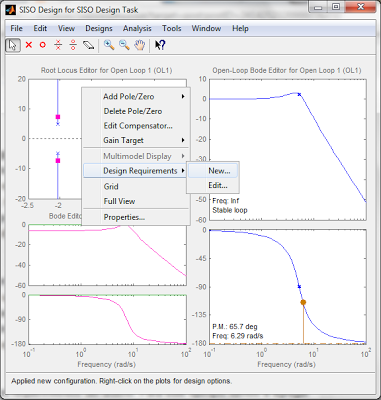
\includegraphics[scale=0.6]{Ventana9}
\renewcommand{\figurename}{Fig.}
\caption{LTI Viewer for SISO Design Task.}
\label{LTI Viewer for SISO Design Task.}
\end{figure}

Los requerimientos que se van a agregar son:

\begin{center}
Settling time = 0.75 \\
Percent Overshoot = 5 \\
\end{center}

Despues de agregar estos requerimientos de diseño la gráfica del LGR queda como se observa en la \textit{Fig. 2.16} \\

\begin{figure}[h]
\centering
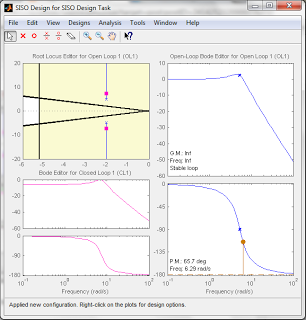
\includegraphics[scale=0.6]{Ventana10}
\renewcommand{\figurename}{Fig.}
\caption{LTI Viewer for SISO Design Task.}
\label{LTI Viewer for SISO Design Task.}
\end{figure}

Al agregar el \textit{“Settling time”} se dibuja una línea vertical  y al agregar el \textit{“Percent Overshoot”} se dibujan dos líneas simétricas sobre el eje real que parten desde el origen con un determinado Angulo y que interceptan la línea dibujada por el \textit{“Settling time”}. Entonces para que se cumplan los requerimientos del diseño los polos dominantes del sistema se deben encontrar en estos puntos de intersección o muy cerca de ellos. Se observa que deben moverse los polos hacia estos puntos, ya que la linea del $LGR$ no pasa por ahí. \\

El proceso de diseño del compensador mediante el método $LGR$ consiste en agregar polos o ceros al compensador para modificar el $LGR$ de tal forma que este pase por los puntos determinados en donde deben estar los polos dominantes para obtener la respuesta deseada. Después de consiguir lo anterior, se arrastran los polos  hasta estos puntos, y entonces la gráfica de la respuesta del sistema debe coincidir con la respuesta deseada. Pero puede que esto no ocurra, y seguramente se debe a que los polos que se ubican en estos puntos no son los dominantes. \\

Para poder predecir los cambios que sufre el $LGR$ al agregar un polo o un cero se debe tener un buen conocimiento de la forma en que se dibuja el $LGR$. Si no se posee este conocimiento se recomienda leer las secciones $6.1$, $6.2$ y $6.3$ del capitulo 6 del libro \textit{Ingeniería de Control Moderna de Ogata}. Las opciones para agregar o quitar polos o ceros están donde indica la \textit{Fig. 2.17}. \\

\begin{figure}[h]
\centering
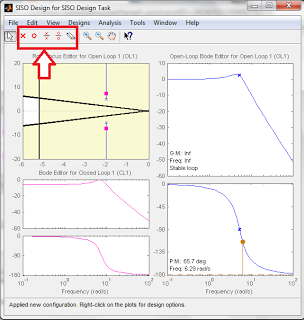
\includegraphics[scale=0.7]{Ventana11}
\renewcommand{\figurename}{Fig.}
\caption{LTI Viewer for SISO Design Task.}
\label{LTI Viewer for SISO Design Task.}
\end{figure}

Se procede a comenzar con el diseño. Para correr los polos hacia la izquierda se agrega un cero en el eje real. Se mueve este cero hasta que el $LGR$ pase por los puntos indicados y se arrastran los polos hasta estos puntos. Despues de hacer esto la gráfica del $LGR$ ha debido quedar como en la \textit{Fig. 2.18}. \\

\begin{figure}[h]
\centering
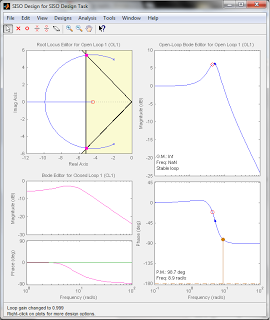
\includegraphics[scale=0.7]{Ventana12}
\renewcommand{\figurename}{Fig.}
\caption{LTI Viewer for SISO Design Task.}
\label{LTI Viewer for SISO Design Task.}
\end{figure}

Y la gráfica de la respuesta del sistema que se muestra con la linea azul contínua ha debido quedar como sigue. \\

\begin{figure}[h]
\centering
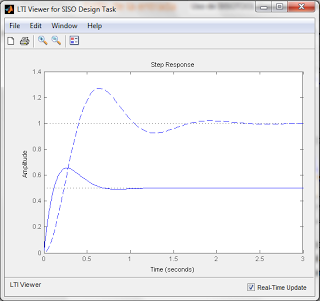
\includegraphics[scale=0.6]{Ventana13}
\renewcommand{\figurename}{Fig.}
\caption{LTI Viewer for SISO Design Task.}
\label{LTI Viewer for SISO Design Task.}
\end{figure}

En esta imagen se puede apreciar que efectivamente  el tiempo de asentamiento de la respuesta del sistema a lazo cerrado ahora se encuentra alrededor se $0.75 segundos$. Aunque no es tan claro que se halla cumplido con el requerimiento del porcentaje de sobrepaso. Como se dijo antes al especificar los requerimientos del diseño, \textit{sisotool} traza una gráfica  sobre el $LGR$ que proporciona una idea de donde deben estar los polos para que el sistema funcione como se desea. Es decir solo da una aproximación. \\

Ya se logro cumplir con el requerimiento de tiempo de asentamiento pero se genero otro problema y es el gran error en estado estacionario que posee ahora el sistema a lazo cerrado. La salida debe asentarse en un valor de $1$ pero lo hace en un valor aproximado de $0.45$. Ahora para corregir el error en estado estacionario se agrega un integrador, es decir un polo en el origen. El $LGR$ y la gráfica de la respuesta del sistema se observan en la \textit{Fig. 2.20}. \\

\begin{figure}[h]
\centering
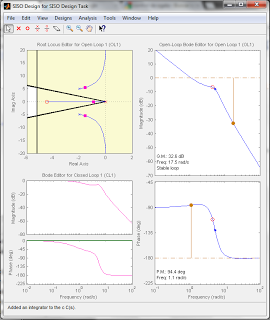
\includegraphics[scale=0.7]{Ventana14}
\renewcommand{\figurename}{Fig.}
\caption{LTI Viewer for SISO Design Task.}
\label{LTI Viewer for SISO Design Task.}
\end{figure}

Tal como se ve, ahora no hay error en estado estacionario pero todo lo demás se altero y la gráfica del $LGR$ se modifico totalmente. Lla gráfica del $LGR$ puede restablecerse a forma parecida a la anterior agregando un cero en el eje real entre el cero que se había agregado antes y el polo en el origen que se agregó ahora, ya que esto obliga a que la parte del $LGR$ que empieza desde el polo en el origen llegue solo hasta el nuevo cero que se agregó. Haciendo esto que los polos complejos conjugados que existían originalmente vuelvan a interactuar de la misma forma que antes con el primer cero que se agregó. Al agregar el nuevo cero el $LGR$ queda como se observa en la \textit{Fig. 2.21}. \\

Como ahora el polo que esta mas cerca al origen fue el que se agregó, los otros dos polos complejos conjugados no son los dominantes, por lo que las gráficas de los requerimientos de diseño ya no son proporcionan confiabilidad. \\

\begin{figure}[h]
\centering
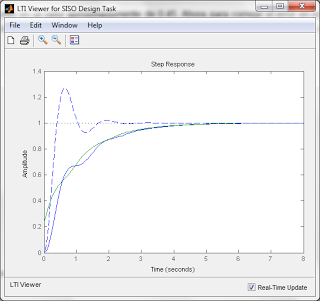
\includegraphics[scale=0.7]{Ventana15}
\renewcommand{\figurename}{Fig.}
\caption{LTI Viewer for SISO Design Task.}
\label{LTI Viewer for SISO Design Task.}
\end{figure}

Como regla general un sistema es mas estable entre más alejados del origen se encuentren sus polos. Así que se corren los polos a la izquierda para ver el resultado. \\

Mientras se mueven los polos hacia la izquierda se llega un punto en el que se obtiene la siguiente gráfica de la \textit{Fig. 2.22} con la respuesta del sistema. \\

\begin{figure}[h]
\centering
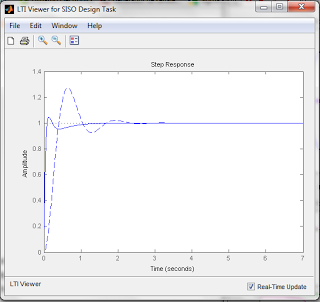
\includegraphics[scale=0.6]{Ventana16}
\renewcommand{\figurename}{Fig.}
\caption{LTI Viewer for SISO Design Task.}
\label{LTI Viewer for SISO Design Task.}
\end{figure}

Como se observa, esta respuesta es bastante mejor de lo que se tenia plantedo inicialmente, pero también pueden ocurrir el caso en que no se logra llegar siquiera a los objetivos planteados inicialmente. Si se siguen moviendo los polos a la izquierda la respuesta seguirá mejorando, pero cuando se hace eso se esta aumentando la ganancia del compensador, y no se podrá implementar un compensador que tenga una ganancia muy elevada. Para ver como queda función de transferencia del compensador se selecciona la opción $"edit$ $compensator"$ del menú \textit{"designs"} y se abre una ventana donde se muestra la ecuación del compensador que se debe utilizar para conseguir la respuesta a la que se ha llegado. Tal como en la \textit{Fig. 2.23}. \\

\begin{figure}[h]
\centering
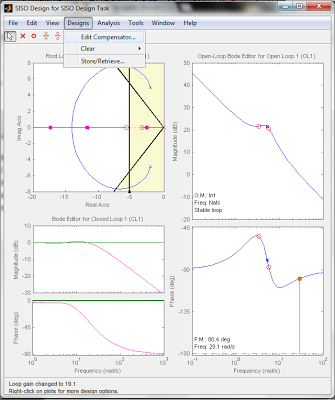
\includegraphics[scale=0.7]{Ventana18}
\renewcommand{\figurename}{Fig.}
\caption{LTI Viewer for SISO Design Task.}
\label{LTI Viewer for SISO Design Task.}
\end{figure}








\newpage





% ==============================================================================================
%												ANEXOS
% ==============================================================================================


\appendix

\chapter{Tarjetas de circuitos impresos}

\section{Historia}

El inventor de los circuitos impresos fue el ingeniero austriaco Paul Eisler (1907-1995) que fabrico el primer circuito impreso alrededor de 1936 como parte de un radio, alrededor  de 1943 los estadunidenses iniciaron el uso de esta tecnología para la fabricación de radios  usados en la segunda guerra mundial, en 1948 se hizo la liberación de la invención tecnológica para que tuviese fines comerciales, pero su mayor impacto fue su fabricación en serie y el proceso de auto-montaje  que fue desarrollado por la  armada de los estados unidos en  1950..
Cuando las tarjetas fueron desarrolladas cada componente electrónico tenía pines de cobre o latón de varios milímetros de longitud, y el circuito impreso tenía orificios taladrados para cada pin del componente. Los pines de los componentes atravesaban los orificios y eran soldados a las pistas del circuito impreso. Este método de ensamblaje es llamado through-hole.
En 1949, Moe Abramson y Stanilus F. Danko, de la armada de  los estados Unidos desarrollaron el proceso de autoensamblaje, en donde las pines de los componentes eran insertadas en una lámina de cobre con el patrón de interconexión, y luego eran soldadas.

\section{Definición}

Una tarjeta de circuito impreso es una superficie conformada por una base de material no conductor y unas pistas o caminos de interconexión de material conductor, estas tarjetas son usadas para interconectar y sostener elementos electrónicos y mecánicos.
Los caminos o pistas son generalmente  de cobre  muestras que la base se fabrica de diferentes resinas de fibra de vidrio.

\section{Normatividad para la construcción de  tarjetas de circuitos impresos}

\subsection{UNE  20-621-84/3}

Esta norma define  los espesores de material aislante para las placas que poseen una o más capas.

\begin{center}
0.2, 0.5, 0.7, 0.8, 1.0, 1.2, 1.5, 1.6, 2.0, 2.4, 3.2, 0 6.4.mm
\end{center}

Las placas que común mente se usan para  tarjetas de una y dos caras conductoras son las  de 2mm, mientras que para las tarjetas multicapas  el espesor depende del número de capas que tenga  y de las hojas de unión entre la misma , los espesores más comunes para tarjetas multicapas son 18, 35, 70 ó 105 um.\\

En esta misma norma  se menciona la forma de interconectar los componentes  a las capas conductoras, estas interconexiones pueden ser de diferentes tipos como lo son:

\begin{enumerate}
\item Agujeros sin metalizar con nudos.
\item Agujeros metalizados con nudos.
\item Agujeros metalizados sin nudos 
\item Nudos sin agujeros (montajes superficiales)
\end{enumerate}

El diámetro de los agujeros depende del componente a usar,  pero en esta norma  se indican los diámetros y la tolerancia de los distintos tipos de agujeros.

\begin{figure}[h]
\centering
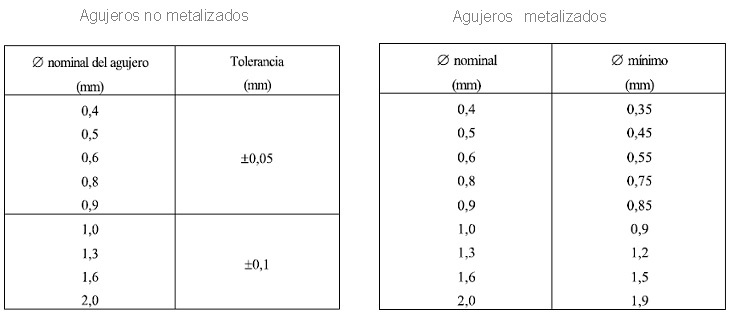
\includegraphics[scale=0.8]{tabla1.jpg}
\renewcommand{\figurename}{Fig.}
\caption{Tipos de agujeros}
\label{Tipos de agujeros}
\end{figure}

Esta misma norma  también define en uno de sus capítulos  el tamaño de las pistas conductoras pues es dependiente  de la corriente eléctrica que va a circular por esta. 
La siguientes graficas presentan las resistencias de las pistas de cobre para diversos espesores de conductores  en función de la anchura de la pista

\begin{figure}[h]
\centering
\includegraphics[scale=0.8]{pistas.jpg}
\renewcommand{\figurename}{Fig.}
\caption{Pistas conductoras}
\label{Pistas conductoras}
\end{figure}

El ancho de la pista se clacula según las especificaciones de corriente que valla a manejar la tarjeta yteniendo en cuenta la siguiente formula:
\begin{equation}
Ancho=\frac{Area}{L*1,378}
\label{Ecu 2}
\end{equation}
\\

\subsection{UNE 20-55-2753}
Esta norma define el tamaño del nudo de soldadura el cual es dependiente del  diámetro del agujero  y su forma, a continuación se muestra las Tabla nominal de nudos y agujeros.

\begin{figure}[h]
\centering
\includegraphics[scale=0.8]{Tabla2.jpg}
\renewcommand{\figurename}{Fig.}
\caption{Tamaño de nudos}
\label{Tamaño de nudos}
\end{figure}

\section{Pautas básicas para la construcción de circuitos impresos}

\begin{enumerate}
\item Hacer el diseño  lo mas sencillo posible, cuanto mas cortas las pistas y mejor sea la distribución de los componentes el resultado será mejor.
\item Realizar el diseño  en una hoja cuadriculada de una décima de pulga, y hacer coincidir las pistas conductoras con las líneas de la cuadricula o hacerlas mismas con Angulo de 45 grados
\begin{figure}[h]
\centering
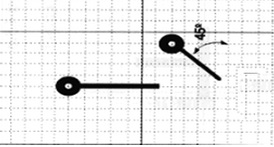
\includegraphics[scale=0.8]{pauta1.jpg}
\renewcommand{\figurename}{Fig.}
\caption{Diseño de pists}
\label{Diseño de pistas}
\end{figure}

\item Cuando se necesite una curva no deben emplearse ángulos de  90 grados, sino anguilos de 135 grados.

 \begin{figure}[h]
 \centering
 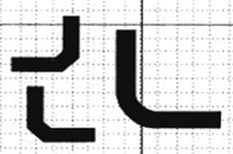
\includegraphics[scale=0.8]{pauta3.jpg}
 \renewcommand{\figurename}{Fig.}
 \caption{Angulos oara el diseño de pistas }
 \label{Angulos oara el diseño de pistas }
 \end{figure}
\item Para realizar bifurcaciones  en una pista conductora, se contemplara realizar triángulos  suavizados.
 \begin{figure}[h]
 \centering
 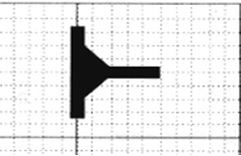
\includegraphics[scale=1.0]{pauta4.jpg}
 \renewcommand{\figurename}{Fig.}
 \caption{Diseño de bifurcaciones entre pistas}
 \label{Diseño de bifurcaciones entre pista }
 \end{figure}
 \item Para conocer e l ancho de la pista  se   debe tener en cuenta el flujo de corriente eléctrica que circulara por la misma.

\begin{enumerate}
\item 1 mm pueden soportar hasta un amperio (1A) de intensidad de corriente
\item 4.5 mm  pueden soportar hasta 10 amperios (10A) de flujo de intensidad de corriente.
\item Las pistas más comunes son las de 2 mm que pueden soportar un promedio de dos amperios (2A) y dependiendo del aspersor podrá 0soportar hasta cinco amperios (5A).	
\end{enumerate}
\item La separación  entre pistas  maneja un estar de 0.8mm pero en diseños complejos se podrá usar una distancia de 0.4mm. cuando se calcule la distancia entre pistas se considerara la tensión eléctrica que habrá entre ellas.La distancia  entre bordes y pistas  será de aproximadamente 5mm
 \begin{figure}[h]
 \centering
 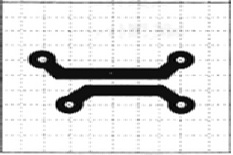
\includegraphics[scale=1.0]{pauta61.jpg}
 \renewcommand{\figurename}{Fig.}
 \caption{Separación entre pistas}
 \label{Separación entre pistas}
 \end{figure}
\item Todos los componentes se pondrán en paralelos a la a los bordes y no se pondrán pistas entre los bordes de la placa
\begin{enumerate}
\item No se pondrán pistas entre dos terminales del cuerpo y componentes activos.
\item Se debe dejar una décima de pulgada  entre el cuerpo del componente y el punto de soldadura correspondiendo en el orificio de la placa.
\begin{figure}[h]
 \centering
 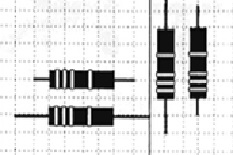
\includegraphics[scale=1.0]{pauta8.jpg}
 \renewcommand{\figurename}{Fig.}
 \caption{Separación entre componentes y pistas}
 \label{Separación entre componentes y pistas }
 \end{figure}
\end{enumerate}
\item En algunas placas de circuitos impresos se pueden usar componentes de tipo SMT que son tarjetas de circuitos impresos pequeñas que se conectan a una tarjeta mayor, existen 4 tipos  las cuales son:
\begin{enumerate}
\item LLC 
\begin{figure}[h]
 \centering
 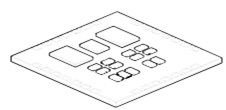
\includegraphics[scale=1.3]{LLC.jpg}
 \renewcommand{\figurename}{Fig.}
 \caption{Placas de circuitos impresos LLC}
 \label{Placas de circuitos impresos LLC}
 \end{figure}
\item SIMM
\begin{figure}[h]
 \centering
 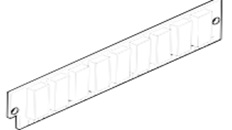
\includegraphics[scale=1.0]{SIMM.jpg}
 \renewcommand{\figurename}{Fig.}
 \caption{Placas de circuitos impresos SIMM}
 \label{Placas de circuitos impresos SIMM}
 \end{figure}\\
   
 \item DIPM
 \begin{figure}[h]
  \centering
  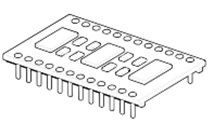
\includegraphics[scale=1.0]{DIP.jpg}
  \renewcommand{\figurename}{Fig.}
  \caption{Placas de circuitos impresos DIP }
  \label{Placas de circuitos impresos DIP}
  \end{figure}
 
  \item SIP
  \begin{figure}[h]
   \centering
   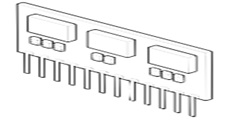
\includegraphics[scale=1.0]{SIP.jpg}
   \renewcommand{\figurename}{Fig.}
   \caption{Placas de circuitos impresos SIP}
   \label{Placas de circuitos impresos SIP}
   \end{figure}
\end{enumerate}
\end{enumerate}

\section{Disposición  De Componentes}

Para la disposición de los  componentes se debe tener en cuenta que hay dos tipos los cuales son:

\begin{enumerate}
\item Componentes de inserción (TDH). En estos componentes se insertan los terminales en los nodos de la placa para posterior soldadura.
\begin{figure}[h]
  \centering
  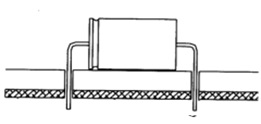
\includegraphics[scale=1.0]{TDH.jpg}
  \renewcommand{\figurename}{Fig.}
  \caption{Componentes en montaje de insercion}
  \label{Componentes en montaje de insercion}
  \end{figure}
\item •	Componentes de montaje superficial (SMD). Son usados  para montajes de alta densidad de componentes
\begin{figure}[h]
  \centering
  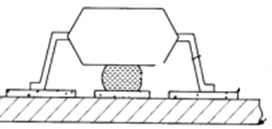
\includegraphics[scale=1.0]{SMD.jpg}
  \renewcommand{\figurename}{Fig.}
  \caption{Componentes en montaje superficial}
  \label{Componentes en montaje Superficial}
  \end{figure}
\end{enumerate}

De acuerdo al tipo de componente  y al tipo de rejillas o agujeros que posea la placa se podrán usar dos tipos de Montale horizontal o vertical, el montaje que se selecciones podrá proporcionar mayor comodidad a la hora de  interconectar y soldar todos los componentes.

\begin{enumerate}
\item	Montaje Vertical
\begin{figure}[h]
  \centering
  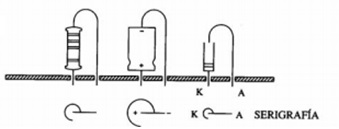
\includegraphics[scale=1.0]{MVERTICAL.jpg}
  \renewcommand{\figurename}{Fig.}
  \caption{Componentes en montaje vertical}
  \label{Componentes en montaje vertical}
  \end{figure}
\item	Montaje Horizontal
\begin{figure}[h]
  \centering
  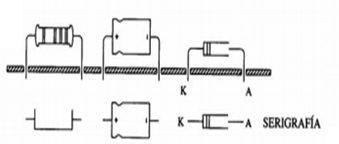
\includegraphics[scale=1.0]{MHORIZONTAL.jpg}
  \renewcommand{\figurename}{Fig.}
  \caption{Componentes en montaje Horizontal}
  \label{Componentes en montaje Horizontal}
  \end{figure}
\end{enumerate}

Una de las prácticas más recomendadas es la separación de componentes análogos de los digitales para evitar problemas  de tamaño, vibración  y resonancia entre los mismo por esta razón se recomienda usar clips de fijación,\\

Para la disposición de los componentes en la placa, estos deben ser fijados  de forma paralela a los ejes X y Y,  pues se debe permitir la identificación  de su código, nomenclatura, valor, etc. \\

\section{Diseño de Pistas}

En todos los circuitos de alimentación están presentes los componentes RLC  y sus corrientes y tensiones parasitas que tienden a desestabilizar la alimentación del circuito.\\

Cuando el circuito se comporta de forma inestable se dice que hay bucles de corriente (corriente de retorno) , para mediar esto y que el circuito de alimentación no se comporte de forma tan inestable es muy importante que el camino de  o trazado de retoño sea directo\\

\begin{figure}[h]
  \centering
  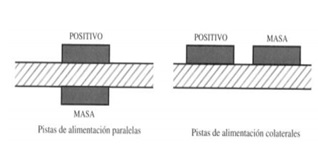
\includegraphics[scale=1.3]{D_PISTAS2.jpg}
  \renewcommand{\figurename}{Fig.}
  \caption{Pistas de alimentación}
  \label{Pistas de alimentación }
\end{figure}

componentes análogos de los digitales pues se deben usar dos pistas de  masa o tierra  totalmente independientes para cada circuito,\\
  
Se debe tratar de que el trazado de  pistas cubra al menos el 50 porciento de  la superficie total de la placa e interconecte todos los componentes necesarios para el correcto funcionamiento.\\

\section{Composición  química}
El atacado químico es el proceso por el cual  pasa el diseño de las pistas  y componentes  a la placa, este se puede producir mediante cloruro férrico (Cl3Fe) o ácido clorhídrico(ClH) y agua oxigenada (H2O2). Este atacadoresponde a las siguientes reacciones:
   
El cloruro férrico se puede adquirir en el mercado especializado en componentes electrónicos, se presenta ya diluido o en forma de sólido granulado.
El ácido clorhídrico y el agua oxigenada se pueden adquirir en diversos comercios y la proporción para la mezcla que realizaremos cada vez que lo vayamos a utilizar (no es reutilizable como el cloruro férrico) es la siguiente:

















\bibliographystyle{IEEEtran}
\bibliography{prueba}
%\printbib{RPFCU-HBB}

\end{document}